\documentclass[11pt]{article}

\usepackage[margin=1in]{geometry}
\usepackage{amsmath}
\usepackage{amssymb}
\usepackage{graphicx}
\usepackage{booktabs}
\usepackage{multirow}
\usepackage{xcolor}
\usepackage{tikz}
\usetikzlibrary{arrows.meta,positioning,shapes.geometric}
\usepackage{hyperref}
\usepackage[numbers,sort&compress]{natbib}

\title{Beyond Forecast Accuracy: Stability-Aware Operational Demand Planning under Execution Constraints}
\author{Author Name Placeholder}
\date{\today}

\begin{document}

\maketitle

\begin{abstract}
Forecast-driven demand planning should be treated as a feasibility-constrained model selection problem rather than a pure forecast accuracy problem. The most accurate forecast is not always the most deployable forecast. This paper studies a decision layer that evaluates forecast accuracy jointly with inventory impact, planning-signal volatility, model switching cost, and execution adaptation burden. Using real retail demand data and supply-chain execution evidence, the empirical analysis tests whether execution risk is measurable and can reorder model deployment choices. Final cross-dataset results will be inserted after the remaining experiments are completed.
\end{abstract}

\section{Introduction}

Demand planning increasingly relies on predictive models to anticipate future demand at fine operational granularity. In many empirical studies and model-selection workflows, the primary criterion for choosing among forecasting methods is numerical prediction accuracy. Metrics such as mean absolute error, root mean squared error, and weighted absolute percentage error are important because inaccurate forecasts can lead to costly overstocking, stockouts, and service failures. However, forecast accuracy alone does not describe whether the resulting plan can be executed.

In real operations, forecasts are not executed directly. A forecast is converted into a planning signal: an inventory target, a replenishment quantity, a labor plan, a production target, a transportation commitment, or an allocation decision. This forecast-to-plan conversion is mediated by business policies, service-level targets, safety-stock rules, system constraints, and planner review processes. The operational question is therefore not only whether a forecast is numerically close to realized demand, but whether the planning signal implied by that forecast is stable, feasible, and worth deploying.

A more accurate forecast may create unstable planning signals. It may require frequent model switching, large period-to-period target jumps, repeated infrastructure updates, or adjustment requests that exceed what suppliers, stores, warehouses, transportation teams, and enterprise planning systems can absorb. These burdens may be invisible in forecast-error tables. A model that looks attractive under WAPE can still be unattractive when it generates plan churn, execution violations, or additional governance work.

This creates a planning-execution gap. Forecasting capability can adapt faster than downstream execution infrastructure. Machine learning pipelines may update daily or weekly, while procurement lead times, labor scheduling, supplier coordination, production planning, and information-system workflows may change more slowly. When the forecasting layer changes faster than the execution layer can absorb, prediction accuracy and deployable planning quality can diverge.

This paper studies forecast-driven demand planning as a feasibility-constrained model selection problem. Rather than asking which forecasting model has the lowest error in isolation, the paper asks which deployable planning strategy balances forecast accuracy, inventory exposure, planning volatility, model-switching burden, and execution-capacity constraints. The objective is not to argue that stability-aware or feasibility-aware strategies always dominate. The objective is to make the tradeoff surface visible and to evaluate model selection in the same operational space where planning decisions are executed.

The empirical design uses three public-data roles. DataCo supply-chain execution data is used to show that execution risk is empirically measurable and to construct data-informed execution-risk sensitivity scenarios. Favorita retail demand data provides the main forecast-to-plan proof of concept, with demand, promotion, holiday, oil-price, transaction, and store-context signals. M5 provides a larger hierarchical retail robustness setting across item, department, category, store, and state levels. Walmart and Rossmann are reserved as optional future robustness extensions; no results from those datasets are claimed in the current draft.

The paper makes four contributions. First, it formulates forecast-driven demand planning as feasibility-constrained model selection, separating forecast generation from the downstream choice of a deployable planning strategy. Second, it defines a normalized planning utility that compares inventory exposure, planning volatility, switching burden, and execution violations relative to an accuracy-first baseline while still reporting raw operational metrics. Third, it constructs DataCo-informed execution-risk scenarios as sensitivity anchors, without claiming exact economic cost calibration between DataCo and the demand-planning datasets. Fourth, it shows empirically that execution-risk-sensitive objectives can reorder deployable strategy rankings and that the preferred deployable method depends on execution scenario, planning granularity, and demand intermittency.

\section{Related Work}

\subsection{Demand Forecasting and Inventory Implications}

Demand forecasting research studies how predictive models can estimate future demand across products, stores, regions, and time periods. A closely related stream connects forecast quality to downstream inventory and service outcomes. This paper builds on that operational motivation but focuses on an intermediate layer that is often left implicit: the conversion of candidate forecasts into planning signals that must be executed under finite adjustment capacity.

% TODO: cite demand forecasting and inventory-control literature.

\subsection{Forecast Combination and Model Selection}

Forecast-combination and model-selection methods provide mechanisms for choosing among or aggregating candidate forecasts. Standard selection criteria often prioritize forecast error on validation data. The present paper differs by evaluating deployable planning utility rather than forecast error alone. A forecast combination can be attractive not only because it improves accuracy, but because it reduces abrupt plan changes, spreads model risk, or avoids unnecessary switching.

% TODO: cite forecast combination and model-selection literature.

\subsection{Cost-Sensitive and Multi-Objective Decision Making}

Cost-sensitive and multi-objective decision methods are related because demand planning rarely has a single objective. Inventory cost, service level, volatility, and execution burden can move in different directions. The contribution here is not a generic multi-objective optimizer. It is a structured operational planning evaluation framework in which forecast-driven plans are compared against execution-capacity constraints and normalized relative to an accuracy-first baseline.

% TODO: cite cost-sensitive learning and multi-objective optimization literature.

\subsection{Supply-Chain Execution Risk and Planning Stability}

Supply-chain execution risk, planning nervousness, and plan volatility are central to the gap studied in this paper. Downstream operations may be unable to absorb large changes in inventory targets, replenishment quantities, transportation commitments, or staffing plans. This paper connects forecast-driven model selection to measurable execution feasibility by using supply-chain execution evidence to define scenario weights and by evaluating planning volatility and execution violations directly.

% TODO: cite supply-chain execution risk, planning nervousness, and volatility literature.

\section{Problem Formulation}

\subsection{Planning Units and Candidate Forecasts}

Let $i$ index a planning unit, such as an item-store or store-family pair, and let $t$ index a planning period. Let $m \in \mathcal{M}$ denote a candidate forecasting model. Actual demand is denoted by $y_{i,t}$, and the forecast produced by model $m$ is denoted by $\hat{y}_{i,t}^{m}$.

The forecasting layer produces a set of candidate forecasts:
\begin{equation}
    \left\{\hat{y}_{i,t}^{m}: m \in \mathcal{M}\right\}.
\end{equation}

The decision layer converts these candidate forecasts into a final forecast signal $\tilde{y}_{i,t}$ and then into an executable planning signal $x_{i,t}$.

\subsection{Hard Model Selection}

Under hard model selection, the decision layer selects one model $z_{i,t} \in \mathcal{M}$ for each planning unit and period:
\begin{equation}
    \tilde{y}_{i,t} = \hat{y}_{i,t}^{z_{i,t}}.
\end{equation}

Hard selection is operationally meaningful because changing $z_{i,t}$ can require model validation, monitoring changes, deployment updates, and planner communication.

\subsection{Soft Model Composition}

Under soft model composition, the decision layer assigns a nonnegative weight $w_{i,t}^{m}$ to each candidate model:
\begin{equation}
    \tilde{y}_{i,t} = \sum_{m \in \mathcal{M}} w_{i,t}^{m}\hat{y}_{i,t}^{m}.
\end{equation}

The weights satisfy:
\begin{align}
    w_{i,t}^{m} &\geq 0, \\
    \sum_{m \in \mathcal{M}} w_{i,t}^{m} &= 1.
\end{align}

Soft composition can reduce hard model switching, but large weight changes may still create governance and monitoring burden.

\subsection{Planning Signal Conversion}

The operation executes a planning signal rather than a raw forecast. In this initial formulation, the planning signal is an inventory target:
\begin{equation}
    x_{i,t} = \tilde{y}_{i,t} + \text{safety\_stock}_{i,t}.
\end{equation}

The same framework can later represent other executable signals, including replenishment quantities, production targets, staffing levels, or capacity allocations.

\subsection{Inventory Cost}

Inventory cost includes holding cost for over-planning and shortage cost for under-planning:
\begin{align}
    \text{holding\_cost}_{i,t} &= h \max(x_{i,t} - y_{i,t}, 0), \\
    \text{shortage\_cost}_{i,t} &= p \max(y_{i,t} - x_{i,t}, 0), \\
    \text{inventory\_cost}_{i,t} &= \text{holding\_cost}_{i,t} + \text{shortage\_cost}_{i,t},
\end{align}
where $h$ is the holding cost rate and $p$ is the shortage cost rate.

\subsection{Planning Signal Volatility}

Planning signal volatility measures how sharply the executable signal changes across periods:
\begin{equation}
    \text{plan\_change\_pct}_{i,t}
    =
    \frac{|x_{i,t} - x_{i,t-1}|}{\max(|x_{i,t-1}|, \epsilon)}.
\end{equation}

This term captures plan churn that may be invisible in forecast error metrics.

\subsection{Model Switching Cost}

For hard selection, model switching cost is:
\begin{equation}
    \text{switch\_cost}_{i,t}
    =
    \begin{cases}
    1, & z_{i,t} \neq z_{i,t-1}, \\
    0, & z_{i,t} = z_{i,t-1}.
    \end{cases}
\end{equation}

For soft composition, the analogous instability measure is total weight movement:
\begin{equation}
    \text{weight\_change}_{i,t}
    =
    \sum_{m \in \mathcal{M}}
    |w_{i,t}^{m} - w_{i,t-1}^{m}|.
\end{equation}

\subsection{Execution Adaptation Penalty}

Let $C_{i,t}$ denote execution capacity, defined as the maximum plan change the operation can absorb in period $t$. The execution adaptation penalty is:
\begin{equation}
    \text{execution\_penalty}_{i,t}
    =
    \max\left(0, |x_{i,t} - x_{i,t-1}| - C_{i,t}\right).
\end{equation}

This penalty captures the planning-infrastructure gap. It becomes positive when the forecast or planning signal changes faster than execution infrastructure can absorb. In practical terms, the forecasting layer may update rapidly, while procurement, staffing, production, transportation, software systems, or planner workflows may only absorb smaller or slower changes.

\subsection{Multi-objective Planning Loss}

The project evaluates planning utility through a multi-objective loss:
\begin{align}
    \text{total\_loss}
    ={}&
    \alpha \cdot \text{forecast\_error}
    + \beta \cdot \text{inventory\_cost} \notag \\
    &+ \lambda_{\text{volatility}} \cdot \text{planning\_signal\_volatility} \notag \\
    &+ \lambda_{\text{switch}} \cdot \text{model\_switching\_cost} \notag \\
    &+ \lambda_{\text{execution}} \cdot \text{execution\_adaptation\_penalty}.
\end{align}

The weighted scalar loss is useful for optimization and policy comparison. The paper will also report Pareto-style multi-objective outputs so that tradeoffs among accuracy, inventory cost, stability, switching, and execution adaptation remain visible.

\section{Framework}

The proposed framework separates forecasting from operational planning decisions. Candidate forecasting models generate demand forecasts. A decision layer then selects or combines these forecasts while accounting for stability, model switching cost, and execution capacity. The selected forecast is converted into a planning signal, such as an inventory target, and evaluated in an operational planning simulator.

The framework is designed to answer whether a forecast that is numerically more accurate also improves executable planning quality. Future experiments will instantiate this framework on public demand datasets and compare direct forecast pass-through policies against stability-aware decision strategies.

The improved decision layer includes feasibility-aware smoothing. Instead of immediately replacing the previous executable plan with a new forecast-driven plan, the planner can adapt gradually with an interpretable smoothing parameter. This mechanism is intended to model execution environments where infrastructure, supplier coordination, staffing, or store operations cannot absorb abrupt period-to-period plan changes.

The framework also includes feasibility-aware ensembles. These strategies combine candidate forecasts with nonnegative weights that sum to one, where the weights can be based on validation forecast accuracy, validation operational loss, or a transparent constrained validation grid. These ensemble variants are included to test whether a soft composition strategy can preserve useful accuracy while reducing execution burden.

Figure~\ref{fig:feasibility-analysis-flowchart} summarizes the planned analysis workflow. The figure is a structural placeholder and does not report empirical findings.

\begin{figure}[htbp]
\centering
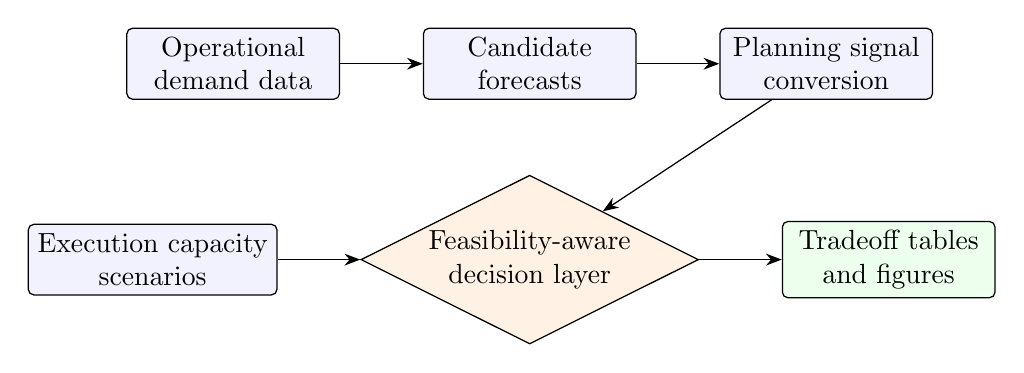
\begin{tikzpicture}[
    node distance=0.95cm and 1.05cm,
    stage/.style={
        draw,
        rounded corners=2pt,
        align=center,
        minimum width=2.7cm,
        minimum height=0.82cm,
        fill=blue!5,
        line width=0.45pt
    },
    decision/.style={
        draw,
        diamond,
        aspect=2.0,
        align=center,
        inner sep=1.2pt,
        fill=orange!10,
        line width=0.45pt
    },
    output/.style={
        draw,
        rounded corners=2pt,
        align=center,
        minimum width=2.7cm,
        minimum height=0.82cm,
        fill=green!7,
        line width=0.45pt
    },
    arrow/.style={-{Stealth[length=2.0mm]}, line width=0.45pt}
]
\node[stage] (data) {Operational\\demand data};
\node[stage, right=of data] (forecasts) {Candidate\\forecasts};
\node[stage, right=of forecasts] (signals) {Planning signal\\conversion};
\node[decision, below=of forecasts] (decision) {Feasibility-aware\\decision layer};
\node[stage, left=of decision] (capacity) {Execution capacity\\scenarios};
\node[output, right=of decision] (outputs) {Tradeoff tables\\and figures};

\draw[arrow] (data) -- (forecasts);
\draw[arrow] (forecasts) -- (signals);
\draw[arrow] (signals) -- (decision);
\draw[arrow] (capacity) -- (decision);
\draw[arrow] (decision) -- (outputs);
\end{tikzpicture}
\caption{Feasibility-aware demand-planning analysis workflow.}
\label{fig:feasibility-analysis-flowchart}
\end{figure}


This section is a placeholder. The final version will describe the implemented pipeline, decision layer variants, feasibility-aware smoothing, feasibility-aware ensembles, execution capacity model, and policy drift scenarios in detail.

\section{Experimental Setup}

\subsection{Datasets}

This subsection is a placeholder for public demand datasets. Candidate datasets include retail, grocery, store-item, and service demand tables with enough history to evaluate rolling planning decisions.

M5 is used as a large-scale hierarchical robustness dataset. It is not treated as a separate forecasting leaderboard task. The M5 robustness analysis uses manually provided local files, converts the wide daily sales table into a long item-store panel, and evaluates whether the Favorita accuracy-feasibility tradeoff persists under larger scale, hierarchy, and intermittent demand.

\subsection{Forecasting Models}

This subsection will describe candidate forecasting models. Initial models may include transparent baselines such as last-value forecasts, rolling averages, seasonal naive forecasts, and later machine learning models.

\subsection{Decision Strategies}

This subsection will describe decision strategies, including forecast pass-through, hard model selection, soft ensemble composition, and stability-aware selection with switching or volatility penalties.

The baseline comparison includes BestAccuracy, Family Best, Feasibility-Aware, Stability-Aware, Simple Ensemble, Best Inventory Cost, Best Stability, and an Oracle upper bound. The Oracle strategy may use realized test-period outcomes and is therefore non-deployable; it is included only as a diagnostic upper bound.

The improved method comparison adds feasibility-aware smoothed planning and feasibility-aware ensemble strategies. Fixed-alpha smoothing, scenario-based alpha smoothing, and utility-based alpha smoothing are evaluated as interpretable gradual-adaptation policies. Utility-based alpha is selected with blocked validation folds to reduce overfitting to a single validation period. Feasibility-aware ensembles include inverse-accuracy weighting, inverse-operational-loss weighting, and a constrained validation-grid ensemble with nonnegative weights that sum to one.

\subsection{Evaluation Metrics}

This subsection will define forecast metrics, inventory metrics, stability metrics, execution adaptation metrics, and the weighted planning utility objective used in the experiments.

Normalized planning loss is reported relative to the accuracy-first BestAccuracy baseline within the same run mode and split. Raw WAPE, inventory cost, planning volatility, execution penalty, violation rate, switch count, and raw total planning loss remain visible in the result tables.

The improved method analysis also reports the maximum period plan change, normalized inventory component, normalized volatility component, normalized execution component, normalized switch component, rank by normalized total loss, rank by WAPE, rank by execution penalty, and gap to the non-deployable Oracle diagnostic.

\subsection{Execution Capacity Scenarios}

This subsection will describe execution capacity stress tests. These scenarios evaluate how planning strategies behave when downstream operations can absorb only limited period-to-period plan changes.

DataCo is used to construct data-informed execution-risk scenarios rather than to directly estimate the exact economic cost of execution violations in the demand-planning datasets. When DataCo late-delivery anchors are unavailable, the pipeline records fallback usage and applies configured default scenario values.

The M5 robustness pipeline reuses the same DataCo-informed execution scenarios when the generated scenario table is available. If the generated table is unavailable, configured fallback scenarios are used and the run log records this explicitly.

\subsection{M5 Robustness Design}

This subsection is a placeholder for the M5 robustness design. The planned analysis includes large-scale replication at item-store level, hierarchy sensitivity across item-store, department-store, and category-store grains, intermittent-demand stress tests, and DataCo-informed execution scenario robustness.

\subsection{Policy and Context Drift Scenarios}

This subsection will describe policy and context drift scenarios, such as changes in service-level targets, shortage costs, lead times, or execution capacity.

\section{Results}

This section is a placeholder. No final experimental results are reported at this stage.

\subsection{Model Heterogeneity Results}

Placeholder for results showing how candidate forecasting models differ across planning units, time periods, or demand regimes.

\subsection{Accuracy versus Inventory Cost}

Placeholder for analysis comparing forecast accuracy improvements against inventory holding and shortage costs.

\subsection{Accuracy versus Planning Volatility}

Placeholder for analysis showing whether more accurate forecasts create larger planning signal changes.

\subsection{Execution Capacity Stress Test}

Placeholder for stress-test results showing when planning signals exceed execution capacity.

\subsection{Policy Drift Results}

Placeholder for results under changing service-level targets, shortage costs, lead times, or execution capacity.

\subsection{Ablation Study}

Placeholder for ablation results isolating the contribution of stability penalties, switching penalties, execution penalties, and safety stock assumptions.

\section{Discussion}

This section will interpret the empirical findings and explain when stability-aware decision layers improve operational planning utility. It will also discuss limitations, generalizability, and implications for planning system design.

\section{Conclusion}

Forecast accuracy remains central to demand planning, but it is not sufficient for deployment. Operational systems execute planning signals, not forecast-error tables. A model that improves WAPE can still create unstable targets, frequent adjustments, switching burden, or execution violations that make the plan less deployable.

This paper formulates forecast-driven demand planning as feasibility-constrained model selection. The framework evaluates candidate strategies using inventory exposure, planning volatility, switching burden, and execution-capacity violations alongside forecast accuracy. DataCo provides an empirical anchor for execution-risk sensitivity, Favorita provides the main forecast-to-plan proof of concept, and M5 provides hierarchical robustness evidence.

The current results show that execution-risk-sensitive objectives can reorder deployable strategy rankings. They also show that the preferred deployable method depends on execution scenario, planning granularity, and demand intermittency. This does not imply that any single feasibility-aware method universally dominates. It supports the narrower and more operationally useful conclusion that feasibility must be evaluated explicitly when forecasting models are selected for planning systems.

The manuscript is intentionally structured as a living draft. Additional Walmart and Rossmann robustness experiments, richer execution-cost calibration, and enterprise workflow evidence can be incorporated without changing the core argument: accurate forecasts become operationally valuable only when they can be converted into feasible plans.


\bibliographystyle{plainnat}
\bibliography{references}

\end{document}
